\section{Instantaneous Velocity}

\makelabheader %(Space for student name, etc., defined in master.tex or labmanual_formatting_commands.tex)

{\noindent \bf Objectives:} 

\begin{itemize}[nosep]
\item To make plausible the idea of velocity at an instant. 
\item To demonstrate that nonuniform motion appears increasingly uniform as the time interval becomes successively shorter. 
\item To understand the notion of ``taking a limit.''
\end{itemize}

\textbf{Apparatus:}

\begin{itemize}
\item Track and cart 
\item Pasco 550 Interface
\item Capstone software (\filename{P\_Graphs.cap} experiment file)
\item Motion detector
\item Lab stand
\end{itemize}
{\noindent \bf Activity 1: An experiment} \begin{enumerate}

\item Open the file \filename{P\_Graphs.cap} in the \filename{\coursefolder} folder.

\item You will release a cart to roll down the track toward the motion
detector. \emph{Stop the cart before it hits the motion detector}. Also, be sure
that you aim the motion detector at the cart and that there are no people or
extraneous objects within a 20 degree cone of the track (with vertex
at the motion detector). Spurious motions within the sensitivity of
the motion detector give false signals.

\item Place the cart near the 2-meter mark at the raised end of the track, opposite that on which the motion detector is mounted.

\item Release the cart from rest and start recording data.

\item A graph with dots at regular \textit{time} intervals will be created on the screen. Stop the cart before it hits the motion detector. You may need to repeat the data taking until you get a reasonable looking chart (see Question 1).

\item Print out a copy of the graph for each member of the lab group.

\end{enumerate}

\medskip

{\noindent \bf Questions:}

1. Describe the distribution of the dots. Are they as you would have expected?
Is the motion it represents uniform or not? Explain. 
\answerspace{20mm}

\pagebreak[2]
2. Select ten data points on your graph ising the \button{highlight} tool. (See Appendix \ref{capstone}.) 
Use the scroll wheel to zoom in until the highlighted data points span the graph.
Notice that zooming in has the effect of viewing the data over successively
shorter time intervals. What does examining the data over successively shorter
time intervals demonstrate? Explain.
\answerspace{20mm}

3. Read the exact coordinates in position and time
for the first and last points highlighted on the graph. (Use the \button{coordinates} tool; see Appendix \ref{capstone}.)  Calculate \( \Delta x/\Delta t \)
and explain the significance of this quantity.
\answerspace{20mm}

{\noindent \bf Discussion} You just approximated the instantaneous velocity for the central point of your section of dots. The instantaneous velocity is the velocity the object would have at a particular instant if it were moving at uniform velocity during the entire interval. You also approximated a derivative: the ratio of the displacement to the time interval as the time interval approaches zero seconds. 

{\noindent \bf Activity 2: A Graphing Exercise} \begin{enumerate}

\item On the next page, you will find three position versus clock reading graphs. The first one depicts motion over an eight second time interval. We want to know the instantaneous velocity at clock reading 3 sec.

\item On the second graph, replot the outlined segment of the first graph, this time magnifying both position and time by a factor of ten.

\item On the third graph, magnify again by a factor of ten the equivalent section of the second graph around clock reading 3 sec and position 16 cm. 

\item If you are satisfied with the straightness of the line in the third graph, calculate $\frac{\Delta s}{\Delta t}$, the average velocity for this interval. Since the line is sufficiently straight, the result of your calculation may be identified also as the instantaneous velocity at the midpoint of the interval.

\item The curve in the first graph depicts the motion of the object. Determine the equation of motion (the equation of the curve).

\item Take the derivative of this equation of motion and evaluate it at the central clock reading of your final interval. This is also a determination of the instantaneous velocity at that clock reading.

\end{enumerate}

\medskip

{\noindent \bf Questions:}

1. Compare your two calculations of the instantaneous velocity. Are they the
same or do they differ? Should they be the same or different? Explain. 
\answerspace{20mm}

2. Plot a line on the first graph through the point (3~s, 16~cm) which has the
slope of the line in the last graph. What is this line in relation to the motion
curve?
\answerspace{20mm}

\pagebreak[2]
%\vspace{0.3cm}
%{\par\centering 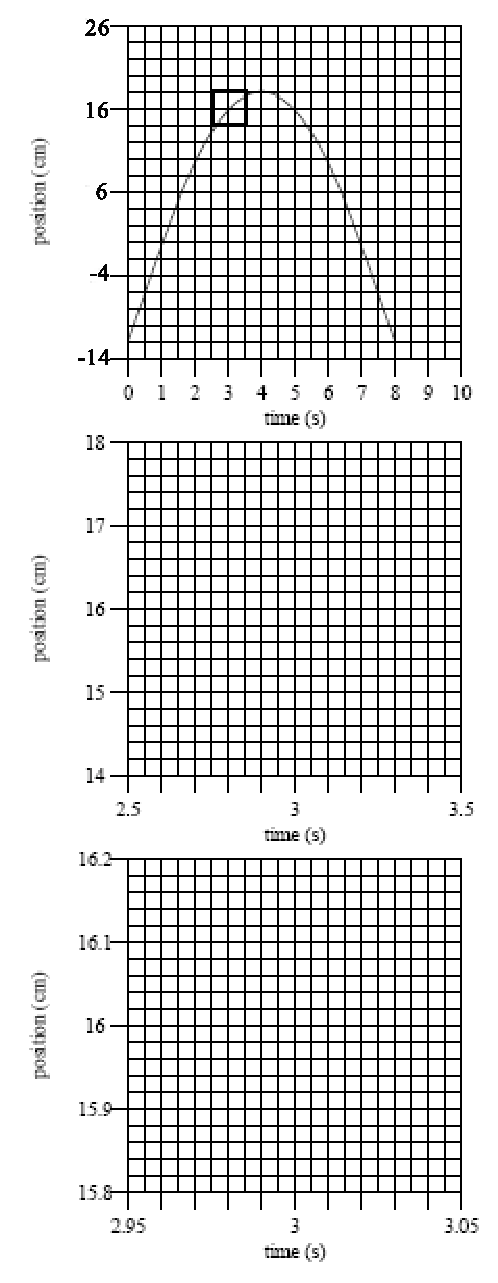
\includegraphics{instantaneous_velocity/instantaneous_velocity_fig1.eps} \par}
%\vspace{0.3cm}

\begin{lab_axis}*[lab_grid,
	height = {3in}, width = {3.0in},
	xlabel={Time (s)},
	ylabel={Position (cm)},
	xmin=0,xmax=10,
	ymin=-14, ymax = 26,
	ytick={-14,-4,6,16,26},
	minor y tick num=4,
	minor x tick num=3,
	]
\addplot coordinates {(2.5,14) (3.5,14) (3.5,18) (2.5,18) (2.5,14) };
\addplot[domain=0:10] {-2*(x-4)^2 + 18} ;
\end{lab_axis}

\begin{lab_axis}*[lab_grid,
	height = {3in}, width = {3.0in},
	xlabel={Time (s)},
	ylabel={Position (cm)},
	xmin=2.5,xmax=3.5,
	ymin=14, ymax = 18,
	minor y tick num=1,
	xtick = {2.5,3.0,3.5},
	minor x tick num=4,
	ylabel_align={-14},
	]
\end{lab_axis}

\begin{lab_axis}*[lab_grid,
	height = {3in}, width = {3.0in},
	xlabel={Time (s)},
	ylabel={Position (cm)},
	xmin=2.95,xmax=3.05,
	ymin=15.8, ymax = 16.2,
	minor y tick num=1,
	xtick = {2.95,3.0,3.05},
	minor x tick num=4,
	ylabel_align={-14},
	]
\end{lab_axis}
